% Multiple Choice Question 22 to 23 (2 questions)

% \par\noindent\rule{0.75\textwidth}{0.5pt} 
\textbf{See the instruction for questions \inteval{\value{question}+1} to \inteval{\value{question}+2}.} 

\begin{center}
    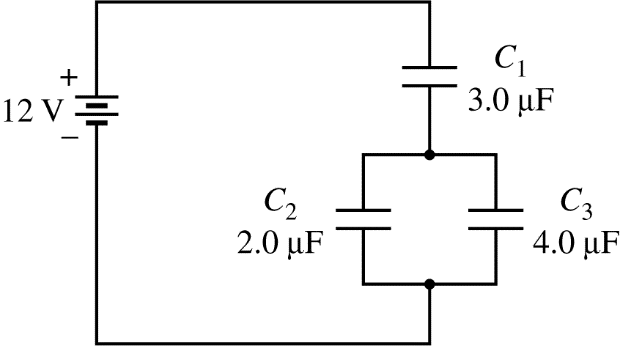
\includegraphics[scale=0.3]{images/img-010-013.png}
\end{center}

The circuit shown above has three capacitors and a $12 \unit{V}$ battery. The capacitors are charged to steady state conditions.

\begin{questions}
\setcounter{question}{21}

% Multiple Choice Question 22
\question
What is the potential difference across capacitor $C_{1}$?

\begin{oneparchoices}
    \choice $3.0 \unit{V}$
    \choice $4.0 \unit{V}$
    \choice $6.0 \unit{V}$
    \choice $8.0 \unit{V}$
    \choice $12 \unit{V}$
\end{oneparchoices}

% Multiple Choice Question 23
\question
One of the capacitors is removed from the circuit and isolated. While it still holds all of its charge, a piece of ceramic with dielectric constant of 2 is inserted and completely fills the space between the plates. $U_{i}$ is the energy stored in the capacitor before the dielectric was inserted, and $U_{f}$ is the energy stored in the capacitor after the dielectric was inserted. What is the ratio $U_{f}/U_{i}$?

\begin{oneparchoices}
    \choice $1/4$
    \choice $1/2$
    \choice $1/1$
    \choice $2/1$
    \choice $4/1$
\end{oneparchoices}

\end{questions}
